% !TEX root =  ../../thesis.tex

\chapter{Bayesian linear mixed effects model}
\label{ch : blmm}

\section{Introduction to linear mixed model}
\label{sec : lmm}
A linear mixed effects model, also known as linear mixed model(LMM) is a statistical model for data which is hierarchical in structure. The specialty of the models is that apart from the fixed effects, they also model the correlation between the observations falling in the same group at a certain level in the hierarchy. The correlation is modeled with the help of random effects and the response is modeled as a linear function of both fixed and random effects.\\

There are many synonymous terminologies for data sets which are hierarchical in nature albeit with subtle nuances differentiating them. In this thesis our focus will be on Longitudinal data sets. A longitudinal data set is the one where multiple observations are collected from subjects at different points in time. For e.g. measurement of Hemoglobin of 20 patients with observations taken every month for a period of 24 months. Since the observations collected from a subject will be correlated a linear model will not be useful because of the restrictions it imposes on the covariance structure.\\

\todo[inline]{Should I mention that Laird and Ware proposed the model?}

\subsection{LMM definition}
\label{subsec : lmm_definition}
Following the notations from \citet{lesaffre_bayesian_2012}, the LMM for the observations of the $i^{th}$ subject among the $n$ subjects is given by\\

$$\boldsymbol{y_i} = \boldsymbol{X}_{i}\boldsymbol{\beta} + \boldsymbol{Z}_{i}\boldsymbol{b}_{i} + \boldsymbol{\varepsilon}_{i}$$\\

where $1 \le i \le n$,\\
$\boldsymbol{y}_i = {(y_{i1}, y_{i2}, \ldots, y_{im_i})}^T$ is a vector of observations for the $i^{th}$ subject taken at $m_i$ time points,\\
$\boldsymbol{X}_i = {(\boldsymbol{x}_{i1}^T, \boldsymbol{x}_{i2}^T, \ldots, \boldsymbol{x}_{im_i}^T)}^T$ is the $m_i \times (d+1)$ design matrix for the $i^{th}$ subject,\\
$\boldsymbol{\beta} = {(\beta_0, \beta_1, \ldots, \beta_d)}^T$ is a $(d+1) \times 1$ vector of fixed effects with $\beta_0$ being the intercept,\\
$\boldsymbol{Z}_i = {(\boldsymbol{z}_{i1}^T, \boldsymbol{z}_{i2}^T, \ldots, \boldsymbol{z}_{im_i}^T)}^T$ is the $m_i \times q$ design matrix of covariates varying for a subject at each observation,\\
$\boldsymbol{b}_i = {(b_{0i}, b_{1i}, \ldots, b_{(q-1)i})}^T$ is a $q \times 1$ vector of random effects with $b_{0i}$ being the random intercept. The random effects $\boldsymbol{b}_i \sim N_q(\boldsymbol{0}, G)$ with $G$ being the $q \times q$ covariance matrix,\\ 
$\boldsymbol{\varepsilon}_{i} = {(\varepsilon_{i1}, \varepsilon_{i2}, \ldots, \varepsilon_{im_i})}^T$ is a $m_i \times 1$ vector of measurement errors. The errors $\boldsymbol{\varepsilon}_{i} \sim N_{m_i}(\boldsymbol{0}, R_i)$ with $R_i$ being the $(m_i \times m_i)$ covariance matrix of errors,\\

The errors $\boldsymbol{\varepsilon}_{i}$ and the random effects $\boldsymbol{b_i}$ are assumed to be independent. $R_i$ is usually a diagonal matrix of the form $\sigma^2I_{m_i}$. While one might only model the correlation between the observations of a subject using random effects, it is also possible to model the serial correlation component. For this and an in depth coverage of LMM we refer the reader to \citet{verbeke_linear_2009}.\\

\section{Motivation for Bayesian linear mixed model}
\label{sec : blmm}
One of issues with the frequentist LMM is that while the parameters in matrices $G$ and $R_i$ are estimated using ML/REML only a point estimate is further used in estimation of fixed effects(see \cite[chap. 5]{verbeke_linear_2009}). Hence the uncertainty in estimation of random effects is ignored. Although frequentist inference approaches try to mitigate this issue by modifying the distributional assumptions of the test statistic \citep[pg. 56]{verbeke_linear_2009}, a bayesian approach considers the variability in parameter estimates in the first place. A similar problem occurs in the estimation of $\boldsymbol{b_i}$. The frequentist strategy is to use Empirical bayes estimates where the the posterior distribution of random effects uses point estimates of parameters in matrices $G$ and $R_i$. Thus the uncertainty in estimation is ignored. On the other hand the bayesian approach averages out over the entire posterior distribution of the hyperparameters to obtain the posterior $p(\boldsymbol{b_i}|\boldsymbol{y})$. In light of these reasons, in this thesis we will model our data using Bayesian linear mixed models.\\

The Bayesian linear mixed model or BLMM can be obtained by assigning a distribution to all the parameters involved in a LMM. This means that for the model presented in section \ref{subsec : lmm_definition} we will have a prior distribution for the following:
\begin{itemize}
\item $\sigma^2 \sim p(\sigma^2)$
\item $\boldsymbol{\beta} \sim p(\boldsymbol{\beta})$
\item $G \sim p(G)$
\end{itemize}

\section{Motivation for mixture of random effects}
As we saw above the random effects are assumed to be multivariate normally distributed. It could be too strong an assumption though in certain cases. A classical example of it are the longitudinal studies where at any time point we would like to categorize subjects in groups. For e.g. group with a high risk of having a certain disease in future vs. group with a low risk. While in retrospective studies it is quite easy as we know exactly which patients were diagnosed with the disease and which were not. However in a study where we would like to categorize patients into different groups well before diagnosis this could be difficult. Here is a toy example for it. Imagine that in longitudinal study we are measuring a response $Y$ which is an indicator of a disease. Assume that from a previous study it is known that patients which are in high risk group for the disease tend to have a higher response $Y$ during all times. Also assume that the trend of $Y$ over time remains the same for both groups otherwise. Figure \ref{fig : random_slope_dummy_data} shows individual profiles of subjects from a simulated dataset. Looking at this plot we can say that a random intercept component will be enough to model individual profiles. Since we will not be knowing which patient belongs to which group, this heterogeneity can be appropriately modeled by considering that the random intercept is a mixture of two normal components.\\

\begin{figure}
	\centering
	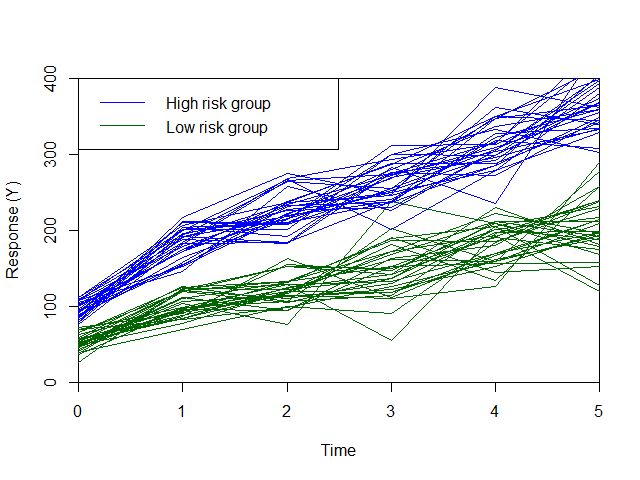
\includegraphics[scale=0.5]{mainmatter/chapter_3_blmm/random_slope_dummy_data.png}
	\caption{Individual profiles of 30 subjects from each group.}
	\label{fig : random_slope_dummy_data}
\end{figure}

In a LMM is quite common to use histogram of Empirical Bayes estimates of random effects to detect groups of individuals. However \citet{verbeke_linear_1996} have shown that if the prior is misspecified(for e.g. if in our example we use a single normal distribution), then it is possible that the histogram of estimates of random effects will be shrunk towards the prior distribution. This means that in our case we may not see a histogram with two distinct modes. The model where a mixture of Gaussian components were used to specify the random effects distribution is called a Heterogeneity model. Various applications of the heterogeneity model can be found in \citet[pg. 264]{fruhwirth-schnatter_finite_2013}.\\

\subsection{Mathematical notation}
Since the random effects are having a Gaussian mixture distribution we will use the following notation to express it mathematically.\\

$$\boldsymbol{b}_i \sim \sum_{k=1}^{K} \eta_k N_q(\boldsymbol{b}_k^C, G_k)$$\\
where $\boldsymbol{b}_k^C$ and $G_k$ are the mean vector and covariance matrices for the $k^{th}$ component in the mixture distribution respectively. The vector $\boldsymbol{\eta} = (\eta_1, \eta_2, \ldots, \eta_K)$ is the weight distribution for the component densities. Since we are following the bayesian paradigm, in addition to prior distribution for $\boldsymbol{\beta}$ and $\sigma^2$ we will now have prior for ($\boldsymbol{b}_1^C, \boldsymbol{b}_2^C, \ldots, \boldsymbol{b}_K^C, \boldsymbol{\eta}, G_1, G_2, \ldots, G_K$).

\section{Parametrization in BLMM}
The random effects $\boldsymbol{b}_i$ in a mixed model could be seen as random deviations from the fixed effects($\boldsymbol{\beta}$) with a mean $\boldsymbol{0}$. For a longitudinal data set, it means that the overall effect of a covariate like time for a subject should be the sum of both fixed and random effects. In this case matrices $\boldsymbol{X}$ and $\boldsymbol{Z}$ both share columns corresponding to the variable time. To enforce the mean $\boldsymbol{0}$ on the random effects in a mixture distribution the following condition should be satisfied.\\

$$E(\boldsymbol{b}_i | \boldsymbol{\phi}) = \sum_{k=1}^{K} \eta_k N_q(\boldsymbol{b}_k^C, G_k) = 0$$,\\
where $\boldsymbol{\phi}$ is the vector ($\boldsymbol{b}_1^C, \boldsymbol{b}_2^C, \ldots, \boldsymbol{b}_K^C, \boldsymbol{\eta}, G_1, G_2, \ldots, G_K$). This further means that $E(\boldsymbol{y}_i | \boldsymbol{\phi}) = \boldsymbol{X}_{i}\boldsymbol{\beta}$. This parametrization which was also used in the original paper on Heterogeneity model \citep{verbeke_linear_1996} is called noncentralized parametrization. The centralized parametrization assumes that the random effects are not deviations from the fixed effects and are centred around a non zero mean. The choice of parametrization has an effect on the rate of convergence while estimating parameters using MCMC. The non-centralized parametrization could be used when within subject heterogeneity is considerably smaller than the heterogeneity due to random effects. Otherwise a centralized parametrization is preferred. We refer the reader to \citet{fruhwirth-schnatter_bayesian_2004} for further details.

\section{Likelihood: Complete data vs Mixture}
The likelihood function in a mixture distribution depends on how much we know about the data. If we know both the data and the allocation vector $\boldsymbol{S}$ then the following likelihood function of parameters is called a complete data likelihood function.\\
$$p(\boldsymbol{y, S}|\boldsymbol{\nu}) = \prod_{i=1}^{N} \prod_{k=1}^{K} (p(\boldsymbol{y}_i | \boldsymbol{\theta}_k) \eta_k)^{I_{S_i=k}}$$\\
where $\boldsymbol{\nu} = (\boldsymbol{\theta}_1, \boldsymbol{\theta}_2, \ldots, \boldsymbol{\theta}_K, \boldsymbol{\eta})$ is a vector of weight distribution and parameters of component densities. It is possible to write this complete data likelihood function in $\perm{K}{K} = K!$ equivalent ways by permuting the order of components. Each order of components is called a Labeling scheme. Although this idea seems trivial we will see ahead that it creates a problem during estimation called label switching. While this likelihood function is valid conditional on knowing the allocation vector $\boldsymbol{S}$, the following likelihood function called Mixture likelihood function applies when we are not aware of the allocations.\\

$$p(\boldsymbol{y}|\boldsymbol{\nu}) = \prod_{i=1}^{N} (\sum_{k=1}^{K} p(\boldsymbol{y}_i | \boldsymbol{\theta}_k) \eta_k)$$\\

It is interesting to note that the mixture likelihood function is symmetrical and has $K!$ modes. We refer readers to \citet[pg. 45-46]{fruhwirth-schnatter_finite_2013} for the review of geometric presentation of this likelihood function.\\

\section{Mixture model identifiability: Label switching}
After running a MCMC procedure to estimate the posterior distributions of the parameters involved, we will be interested in knowing the parameters for the component densities. In most cases we will also be interested in classification of observation using allocation probabilities $P(S_i = k | \boldsymbol{y})$. Now let us imagine that we fitted exactly the true number of components ($K^{true}$ from which the mixture density was formed. At this point it is possible that the posterior densities of parameters do not reflect the true posterior distribution due to label switching.\\

To idea of label switching could be explained with this simple example. Suppose we have a mixture distribution $0.5N(5,1) + 0.5N(7,1)$of two components $C_1$ and $C_2$ and we sampled a few observations from it. The MCMC procedure we will estimate parameters using data augmentation. i.e. we begin with some random allocation vector $\boldsymbol{S}^0$ and estimate parameters using complete data likelihood. For MCMC labels $\mu_1$ and $\mu_2$ exist rather than  $\mu_{C1}$ and $\mu_{C2}$ and it does not associate labels with actual components. We begin with a vague joint prior for these parameters $p(\mu_1, \mu_2) = p(\mu_1)*p(\mu_2) = p(\mu_1)*p(\mu_1) = p(\mu_2)*p(\mu_2)$.\\

Assume that the allocation vector we began with assigns all observations from component $C_1$ to label 1 and all observations from component $C_2$ to label 2. Under such a scheme $(\mu_1,\mu_2) = (5,7)$ is likely. However if we take a conjugate of this allocation vector $(\mu_1,\mu_2) = (7,5)$ will also be accepted. This because we have a mixture likelihood function which is bimodal. Now let us imagine a scenario where because of our initial allocation vector, parameter estimates are $(\mu_1, \mu_2) = (5.5,6.5)$. So far it seems $\mu_1$ represents $\mu_{C1}$ and $\mu_2$ represents $\mu_{C2}$. Now we estimate allocation vector conditional on these estimates in MCMC. Supposing that an observation with value 6.5 originally from component $C_2$ gets allocated to component $C_1$ and similarly an observation with value 5.5 from component $C_1$ gets allocated to $C_2$. Unless we impose some constraint like $\mu_1 < \mu_2$, under the current situations even $(\mu_1,\mu_2) = (6.5, 5.5)$ could be sampled by MCMC. This because under the mixture likelihood it is also likely. However this scenario could've been unlikely if the true means were very far apart. In our scenario the issue is that posterior for $\mu_1$ will have a multiple modes. Not only that but if the sampler kept on arbitrarily switching between the two equivalent posterior regions then both regions will be partially explored. Thus any inference based on this posterior will be useless. \citet[pg. 82]{fruhwirth-schnatter_finite_2013} suggest to use a balanced label switching, which gives multimodal posterior albeit with a full exploration.\\

It is interesting that if our prior for the parameters was not vague, but exactly equal to the true distribution of parameters then label switching might not have happened. However the problem with a strong prior is that an incorrect strong prior could also inadvertently cause label switching or it might not allow a complete exploration of the posterior. Other techniques to stop label switching are imposing an identifiability constraint, which in our case was $\mu_1 < \mu_2$. However in higher dimensions it could become difficult to find a constraint which imposes a unique labeling scheme. For more details we refer the reader to \citet{stephens_dealing_2000}.\\

\section{Mixture model identifiability: Equal or empty components}
A mixture model will also be unidentified if we have an empty component or two components with the same parameters. Suppose the true number of components is $K^{true}$ and we fit $K = K^{true} + 1$ components. In the MCMC sampler suppose one of the components is assigned any observation. Thus the posterior for the parameters will remain the same as the prior. Assuming that the prior for weight distribution $\boldsymbol{\eta}$was a Dirichlet prior $\mathcal{D}(0.5, 0.5, \ldots, 0.5)$, then we will have a posterior for $\boldsymbol{\eta}$ such that the $K^{th}$ component will always have an almost 0 weight in the mixture distribution. This means that at the end of MCMC sampling the component density's posterior will be same as its prior and no observations will be allocated to the component. In such cases the true number of components could be estimated by the count of components with non zero number of allocations. However this situation could be avoided with a stronger prior on the weight distribution which forces the posterior distribution of $\boldsymbol{\eta}$ to be such that no components are empty at the end of MCMC sampling. Identification of number of components in such case is explained in the next section.\\

\textcolor{red}{Gosh! I should explain it in terms of pulling away the posterior eta from the boundary where components of eta are linearly dependent.}. 

\todo[inline]{Should I also discuss the choice of prior?}

\section{Choosing the right number of mixture components}
In most cases we do not know the right number of mixture components in advance unless we have some expert knowledge available or we know them from a previous/similar study. As part of this thesis we will compare many of the existing methods for finding the right number of mixture components.\\

\subsection{Information criteria based methods}
Information criteria are used to select models with parimony and good predictive power. Some of information criteria proposed in the literature are AIC proposed by Akaike, BIC (a minor modification of Schwarz's original criteria), DIC. While AIC and BIC are primarily used in frequentist statistics as they use point estimates of the parameters, DIC follows a more bayesian approach. Following are the definitions of the three criteria:\\

\begin{itemize}
\item $AIC = -2log(p(\boldsymbol{y}|\boldsymbol{\hat{\theta}})) + 2p$
\item $BIC = -2log(p(\boldsymbol{y}|\boldsymbol{\hat{\theta}})) + log(N)p$
\item $DIC = -2log(p(\boldsymbol{y}|\boldsymbol{\bar{\theta}})) + 2p_{DIC}$\\
where $\boldsymbol{\bar{\theta}} = E(\boldsymbol{\theta}_{post}|\boldsymbol{y})$,\\
$p_{DIC} = -2(E(log(p(\boldsymbol{y}|\boldsymbol{\theta}_{post}))) - log(p(\boldsymbol{y}|\boldsymbol{\bar{\theta}})))$ is the penalty for model complexity.
\end{itemize}

It is interesting to mention that the hierarchical nature of the mixture model implies a marginal model as well, which can be found by integrating out the random effects. \citet{verbeke_linear_1996} in their paper on heterogeneity model estimate the fixed effects and all covariance components using this marginal model. In our case y has a marginal model given by:\\

$$\boldsymbol{y_i} \sim \sum_{k=1}^{K} \eta_k N(\boldsymbol{X}_{i}\boldsymbol{\beta} + \boldsymbol{Z}_{i}\boldsymbol{b}_k^C,\boldsymbol{Z}_{i}G_{\boldsymbol{S}_i}\boldsymbol{Z}_{i}^T + R_i)$$\\

If our likelihood function is based on the marginal model then DIC could be used to select models which have good predictive power for an observation which is not necessarily from a subject who is in the current study. The total number of terms which will be penalized by AIC is equal to $dim(\boldsymbol{\eta}) + dim(\boldsymbol{\beta}) + dim(\boldsymbol{b}_{1}^C) + \ldots + dim(\boldsymbol{b}_{K}^C) + dim(G_1) + \ldots + dim(G_K) + 1(for \sigma^2)$, where dim is the total number of elements in the vector or matrix. On the other hand if we stick to the hierarchical interpretation, then DIC could be used to select models which have good predictive power for an observation which has to be from the current set of subjects. The total number of terms which will be penalized by AIC is equal to $dim(\boldsymbol{\beta}) + dim(\boldsymbol{b}_1) + \ldots + dim(\boldsymbol{b}_n) + 1(for \sigma^2)$. A model.

\subsection{Trans Dimensional Bayesian inference}
To compare a set of competing models $\mathcal{M}_1, \mathcal{M}_2, \ldots, \mathcal{M}_{K_{max}}$ each with their own set of parameters $\boldsymbol{\nu}_1, \boldsymbol{\nu}_2, \ldots, \boldsymbol{\nu}_{K_{max}}$ trans dimensional MCMC methods can be used. For e.g. Product space MCMC methods try to simultaneously sample the posterior probability $p(\mathcal{M}_{k}, \boldsymbol{\nu}_1, \boldsymbol{\nu}_2, \ldots, \boldsymbol{\nu}_{K_{max}}, \boldsymbol{y}$ for all $K_{max}$ models. The idea is that during each run a model indicator $\mathcal{M}$ which could follow for e.g. a multinomial distribution, is sampled. Suppose the model indicator is $M=2$ then all the parameters $\boldsymbol{\nu_{2}}$ are sampled whereas parameters for other models are kept what they were. The marginal posterior probability $p(\mathcal{M}_k|\boldsymbol{y}$ of the $k^{th}$ model is found by integrating out the parameters from the joint posterior. These could be further compared to select one of the K models.\\

\subsubsection{Marginal likelihood}
The ratio of marginal posterior could also be expressed as a Bayes Factor (assuming the prior probabilities for both models are equal) which is a ratio of Marginal likelihoods $\dfrac{p(\boldsymbol{y}|\mathcal{M}_i}{p(\boldsymbol{y}|\mathcal{M}_j}$ for the models. 
However \citet{johannes_berkhof_bayesian_2003} also suggest to use goodness of fit measures to be used along with Bayes factor. This because bayes factor is a relative measure. Relying on it completely could lead to selection of a model which is relatively better but overall does not provide a good fit.

\subsection{Posterior predictive checks}


\subsection{Other methods}
We will also explore other graphical methods or informal methods like method of moments in this thesis. For further reading on them we refer the reader to \citet[pg. 107-114]{fruhwirth-schnatter_finite_2013}